\chapter{节点在忙期时队列状态$Q \to P$的马尔可夫链建模与概率生成函数推导}
\label{app:proof_lemma2}
%\addcontentsline{toc}{chapter}{忙期服务过程 ($Q \to P$) 的详细推导}

本附录研究节点忙期内的队列状态演化过程。为此，我们构建一个马尔可夫吸收链模型。模型描述从忙期开始队列长度 $Q$ 到忙期结束队列长度 $P$ 的随机变化。
在此基础上，推导 $G_P(z)$ 与 $G_Q(z)$ 的解析关系。

\section{吸收马尔可夫链模型的构建}

为刻画忙期内队列变化与终止机制，我们定义二维随机过程 $\{(L_t,K_t),t=0,1,\dots\}$。
其中
\begin{itemize}
	\item $L_t \in \{0,1,\dots\}$ 表示节点第 $t$ 次传输尝试开始时的剩余队列长度，但不包含正在发送的数据包。若忙期开始时总队列长度为 $Q$，则有 $L_0=Q-1$。这是因为 HoL~数据包已占用信道。
	\item $K_t \in \{0,1\}$ 表示信道状态。$K_t=1$ 表示忙期保持，即本次传输成功并继续发送，节点保持在忙期。$K_t=0$ 表示节点忙期终止，即发生碰撞或发送结束。
\end{itemize}

如图 \ref{fig:absorbing_markov} 所示，该过程可表示为马尔可夫吸收链。
其状态空间划分如下
\begin{itemize}
	\item \textbf{瞬态} $\mathcal{S}_T=\{(j,1)\mid j\ge 0\}$，表示节点持续成功发送，队列中仍有 $j$ 个待发包。系统处于瞬态时，忙期继续。
	\item \textbf{吸收态} $\mathcal{S}_A=\{(j,0)\mid j\ge 0\}$，表示因碰撞或缓存队列清空而终止忙期。进入该状态后发送过程停止，此时的剩余队列长度即为 $P$。
\end{itemize}

\begin{figure}[htbp]
	\centering
	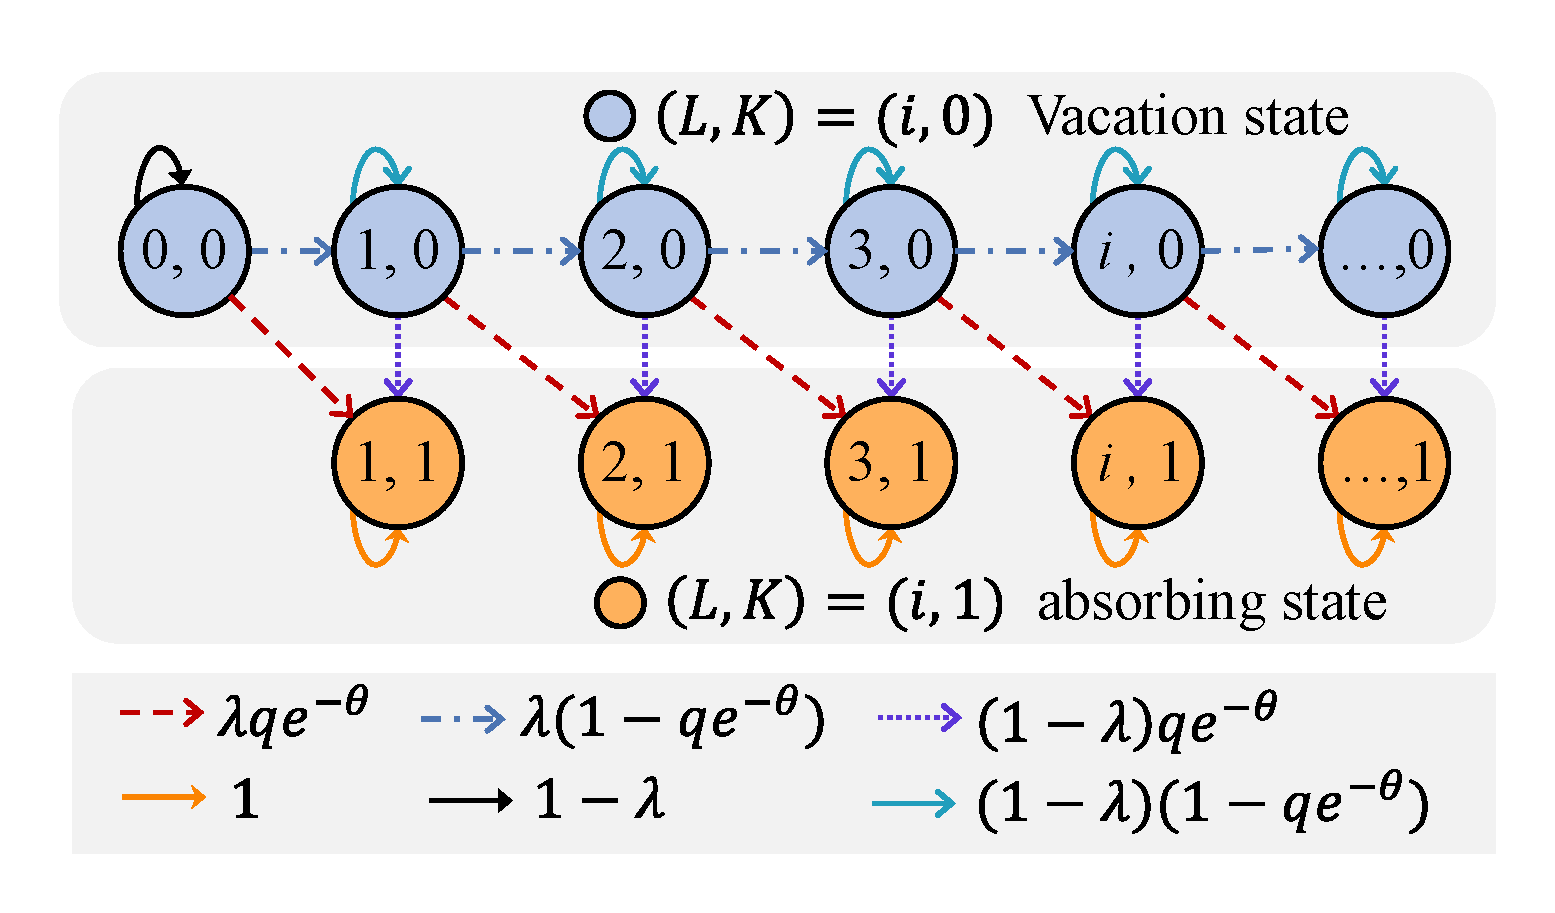
\includegraphics[width=0.8\textwidth]{figure/appdix/P2Q_Absorbing_Markov_chain.pdf}
	\caption{描述忙期内队列演化的吸收马尔可夫链状态转移图}
	\label{fig:absorbing_markov}
\end{figure}

\section{状态转移概率分析}

考虑系统处于瞬态 $(j,1)$。
此时节点正在发送一个数据包，缓存中还有 $j$ 个包。
在一个时隙内，有两类独立过程
\begin{enumerate}
	\item \textbf{新包到达过程}：以概率 $\lambda$到达新包，以概率 $1-\lambda$ 无新包到达。
	\item \textbf{传输过程}：传输成功，即其他 $n-1$ 个节点保持静默的概率为 $e^{-\theta}$；传输失败，即发生碰撞的概率为 $1 - e^{-\theta}$。
\end{enumerate}

综合上述两个过程，下一时刻存在四种转移情形

\begin{enumerate}
	\item \textbf{成功且有新到达}：概率为 $\lambda e^{-\theta}$。发送成功使队列减 1，新包到达使队列加 1。队列长度不变，状态由 $(j,1)$ 转移到 $(j,1)$。
	\item \textbf{成功且无新到达}：概率为 $(1-\lambda)e^{-\theta}$。发送成功且无补充，队列长度减 1。状态由 $(j,1)$ 转移到 $(j-1,1)$。
	\item \textbf{失败且有新到达}：概率为 $\lambda(1-e^{-\theta})$。碰撞使忙期立即结束，新包已进入缓存。状态由 $(j,1)$ 转移到吸收态 $(j+1,0)$。
	\item \textbf{失败且无新到达}：概率为 $(1-\lambda)(1-e^{-\theta})$。碰撞结束忙期且无新包。状态由 $(j,1)$ 转移到吸收态 $(j,0)$。
\end{enumerate}

\section{转移矩阵与基本解}

设忙期开始时队列长度为 $Q$。
当 $Q=1$ 时，系统直接进入吸收态 $(0,0)$，即 $P=0$。
当 $Q\ge 2$ 时，系统从瞬态 $( Q-1,1)$ 出发。
为求吸收概率，我们将状态空间截断为有限维。先设最大队列长度为 $J$，再令 $J\to\infty$。转移矩阵 $\mathbf{M}$ 的标准分块形式为
\begin{equation}
	\mathbf{M} =
	\begin{pmatrix}
		\mathbf{T} & \mathbf{R} \\
		\mathbf{0} & \mathbf{I}
	\end{pmatrix}.
\end{equation}
其中：
\begin{itemize}
	\item $\mathbf{T}$ 是描述瞬态间转移的子矩阵（下双对角矩阵），元素 $t_{j,j} = \lambda e^{-\theta}$，$t_{j, j-1} = (1-\lambda)e^{-\theta}$。
	\item $\mathbf{R}$ 是描述从瞬态进入吸收态的子矩阵，元素 $r_{j, j+1} = \lambda(1-e^{-\theta})$，$r_{j, j} = (1-\lambda)(1-e^{-\theta})$。
\end{itemize}

根据吸收马尔可夫链理论，从任意瞬态 $s_i$ 出发最终被吸收态 $s_j$ 吸收的概率 $b_{ij}$ 构成的吸收概率矩阵为
$$
\mathbf{B}=(\mathbf{I}-\mathbf{T})^{-1}\mathbf{R}.
$$
利用 $\mathbf{T}$ 的下三角结构，可递归求解该矩阵方程。
于是可得从 $( Q-1,1) $ 出发被吸收到 $\langle k,0\rangle$ 的概率，即条件概率 $\Pr\{P=k\mid Q\}$。

经过代数运算，我们得到如下解析解：

\begin{enumerate}
	\item 当 $Q=1$ 时：
	\begin{equation}
		\Pr\{P=0 \mid Q=1\} = 1.
	\end{equation}
	
	\item 当 $Q \ge 2$ 时，对于 $0 \le k \le Q$：
	\begin{equation}
		\Pr\{P=k \mid Q\} = 
		\begin{cases}
			\left[ \frac{(1-\lambda)e^{-\theta}}{1-\lambda e^{-\theta}} \right]^{Q-1}, & k=0 \\
			\frac{(1-\lambda)(1-e^{-\theta})}{1-\lambda e^{-\theta}} \left[ \frac{(1-\lambda)e^{-\theta}}{1-\lambda e^{-\theta}} \right]^{Q-2}, & k=1 \\
			\dots & \vdots \\
			\frac{\lambda(1-e^{-\theta})}{1-\lambda e^{-\theta}}, & k=Q
		\end{cases}
	\end{equation}
\end{enumerate}

\section{PGF关系的建立}

上述条件分布形式较复杂。
在大系统极限下，即 $n\to\infty$ 且 $\lambda\to0$，可利用 PGF 性质得到更简洁表达。
$P$ 表示队列在多次成功发送与新包到达后，被碰撞事件截断时的状态。
据此可证明 $G_P(z)$ 与 $G_Q(z)$ 满足
\begin{equation}
	\label{eq:pgf_P_appendix}
	G_P(z) = G_Q(e^{-\theta}) + \frac{1 - e^{-\theta}}{e^{-\theta} - z} \left[ G_Q(e^{-\theta}) - G_Q(z) \right].
\end{equation}
该式直观地反映了忙期过程对队列分布的过滤作用：$e^{-\theta}$ 项对应于传输成功的概率流，而分母中的 $e^{-\theta}-z$ 项则体现了队列长度随时间步的演化特征。这一结论直接支持了正文中关于 $p_0 = G_P(0)$ 的闭式求解。
